\documentclass[12pt]{amsart}

\usepackage{tikz}
\usepackage{bbm}
\usetikzlibrary{3d,arrows,calc,positioning,decorations.pathreplacing,matrix} %,arrows.meta}

\usepackage{calligra,mathrsfs}
\usepackage[all]{xy}
\usepackage{float, comment}
\usepackage{mathtools}
\usepackage{amsmath}
\usepackage{amsthm}
\usepackage{amssymb}
\usepackage{amsbsy}
\usepackage{amstext}
\usepackage{amsopn}
%\usepackage{mathrsfs} % allows \mathscr
\usepackage[mathscr]{eucal}
\usepackage{enumerate}
\usepackage{xcolor}
\usepackage{graphicx} % allows \includegraphics{}s
\usepackage{scalerel}
\usepackage{microtype} % improves formattings
\usepackage[margin=1in,marginparwidth=0.8in, marginparsep=0.1in]{geometry}
\renewcommand{\baselinestretch}{1.2} % changes page formatting
\usepackage[pagebackref, bookmarks=true, bookmarksopen=true, bookmarksdepth=3,bookmarksopenlevel=2, colorlinks=true, linkcolor=blue, citecolor=blue, filecolor=blue, menucolor=blue, urlcolor=blue]{hyperref}
% \usepackage{newtxtext} % improves font appearance
\usepackage{tikz}
\usepackage{bbm}
\usepackage[all]{xy}
\usetikzlibrary{arrows,calc,positioning,decorations.pathreplacing} %,arrows.meta}

\numberwithin{equation}{section}
\newtheorem{Theorem}[equation]{Theorem}
\newtheorem{Proposition}[equation]{Proposition} 
\newtheorem{Lemma}[equation]{Lemma}
\newtheorem{Open}[equation]{Open Question}
\newtheorem{Corollary}[equation]{Corollary}
\newtheorem{Conjecture}[equation]{Conjecture}
\newtheorem{Specialthm}{Theorem}
\newtheorem{Question}{Question}

\theoremstyle{definition}
\newtheorem{Remark}[equation]{Remark}
\newtheorem{Example}[equation]{Example}
\newtheorem{Definition}[equation]{Definition}

\numberwithin{figure}{section}

\def\la{\langle}
\def\ra{\rangle}
\def\ttimes{\widetilde{\times}}
\def\tbox{\widetilde{\boxtimes}}
\def\bbox{{\boxtimes}}
\def\O{\mathcal{O}}
\def\K{\mathcal{K}}
\def\bG{\mathbb{G}}
\newcommand{\gr}{\mathrm{gr}}
\newcommand{\wt}{\text{wt}}
\newcommand{\mb}[1]{\mathbf{#1}}
\newcommand{\fsl}{\mathfrak{sl}}
\newcommand{\fg}{\mathfrak{g}}
\newcommand{\fn}{\mathfrak{n}}
\newcommand{\bk}{{\mathbbm k}}
\newcommand{\A}{\mathbb{A}}
\newcommand{\C}{\mathbb{C}}
\newcommand{\D}{\mathbb{D}}
\newcommand{\E}{\mathbb{E}}
\newcommand{\G}{\mathbb{G}}
\newcommand{\bN}{\mathbb{N}}
\renewcommand{\P}{\mathbb{P}}
\newcommand{\Q}{\mathbb{Q}}
\newcommand{\Z}{\mathbb{Z}}
\newcommand{\bfC}{{\mathbf{C}}}
\newcommand{\bfD}{{\mathbf{D}}}
\newcommand{\bfI}{{\mathbf{I}}}
\newcommand{\cA}{\mathcal{A}}
\newcommand{\cB}{\mathcal{B}}
\newcommand{\cC}{\mathcal{C}}
\newcommand{\cD}{\mathcal{D}}
\newcommand{\cE}{\mathcal{E}}
\newcommand{\cF}{\mathcal{F}}
\newcommand{\cG}{\mathcal{G}}
\newcommand{\cH}{\mathcal{H}}
\newcommand{\cK}{\mathcal{K}}
\newcommand{\cL}{\mathcal{L}}
\newcommand{\cM}{\mathcal{M}}
\newcommand{\cN}{\mathcal{N}}
\newcommand{\cO}{\mathcal{O}}
\newcommand{\cP}{\mathcal{P}}
\newcommand{\cQ}{\mathcal{Q}}
\newcommand{\cR}{\mathcal{R}}
\newcommand{\cS}{\mathcal{S}}
\newcommand{\cT}{\mathcal{T}}
\newcommand{\cU}{\mathcal{U}}
\newcommand{\cV}{\mathcal{V}}
\newcommand{\cW}{\mathcal{W}}
\newcommand{\cX}{\mathcal{X}}
\newcommand{\cY}{\mathcal{Y}}
\newcommand{\sW}{\mathscr{W}}
\newcommand{\sX}{\mathscr{X}}
\newcommand{\sY}{\mathscr{Y}}
\newcommand{\sZ}{\mathscr{Z}}

\newcommand{\hs}{\heartsuit}
\newcommand{\bul}{\bullet}
\newcommand{\ga}{\gamma}
\newcommand{\al}{\alpha}
\newcommand{\be}{\beta}

%% code from mathabx.sty and mathabx.dcl
\DeclareFontFamily{U}{mathx}{\hyphenchar\font45}
\DeclareFontShape{U}{mathx}{m}{n}{
	<5> <6> <7> <8> <9> <10>
	<10.95> <12> <14.4> <17.28> <20.74> <24.88>
	mathx10
}{}
\DeclareSymbolFont{mathx}{U}{mathx}{m}{n}
\DeclareFontSubstitution{U}{mathx}{m}{n}
\DeclareMathAccent{\widecheck}{0}{mathx}{"71}
\DeclareMathSymbol{\shortminus}{\mathbin}{AMSa}{"39}

\DeclareRobustCommand{\SkipTocEntry}[5]{}

\newcommand{\arrtip}{latex'}

\begin{document}
\title{Notes on Schubert Calculus and Quantum Integrability}

\begin{abstract}
\end{abstract}

\maketitle

\setcounter{tocdepth}{1}

\tableofcontents

\section{Introduction}

\thispagestyle{empty}

Here is a template for a simple commutative diagram in tikz:
\begin{equation*}
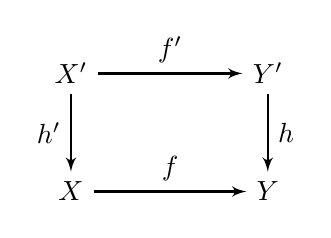
\begin{tikzpicture}
[baseline=(current  bounding  box.center),thick,>=\arrtip]
\node (a) at (0,0) {$X'$};
\node (b) at (2.5,0) {$Y'$};
\node (c) at (0,-1.5) {$X$};
\node (d) at (2.5,-1.5) {$Y$};
\draw[->] (a) to node[above] {$f' $} (b);
\draw[->] (b) to node[right] {$h $} (d);
\draw[->] (a) to node[left] {$h' $}(c);
\draw[->] (c) to node[above] {$f $} (d);
\end{tikzpicture}
\end{equation*}

Here is a template for an elaborate commutative diagram in tikz:
\begin{equation*}
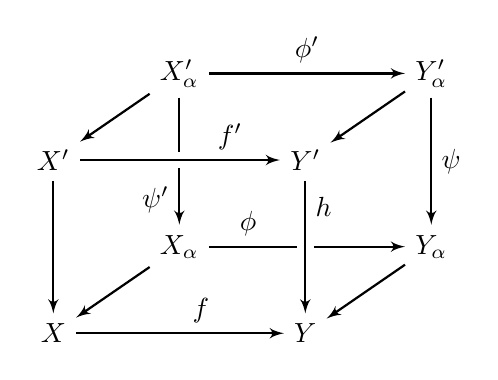
\begin{tikzpicture}[baseline=(current  bounding  box.center),thick,>=\arrtip]
\newcommand*{\ha}{1.6}; \newcommand*{\hb}{1.6}; \newcommand*{\hc}{1.6};
\newcommand*{\va}{-1.1}; \newcommand*{\vb}{-1.1}; \newcommand*{\vc}{-1.1};
\node (ab) at (\ha,0) {$X_\al'$};
\node (ad) at (\ha+\hb+\hc,0) {$Y_\al'$};
\node (ba) at (0,\va) {$X'$};
\node (bc) at (\ha+\hb,\va) {$Y'$};
\node (cb) at (\ha,\va+\vb) {$X_\al$};
\node (cd) at (\ha+\hb+\hc,\va+\vb) {$Y_\al$};
\node (da) at (0,\va+\vb+\vc) {$X$};
\node (dc) at (\ha+\hb,\va+\vb+\vc) {$Y$};
\draw[->] (ab) to node[above] {$\phi' $} (ad);
\draw[->] (ab) to node[above] {$ $} (ba);
\draw[->] (ab) to node[left,pos=.8] {$\psi' $} (cb);
\draw[->] (ad) to node[above] {$ $} (bc);
\draw[->] (ad) to node[right] {$\psi $} (cd);
\draw[->] (ba) to node[above] {$ $} (da);
\draw[->] (cb) to node[above,pos=.2] {$\phi $} (cd);
\draw[->] (cb) to node[above] {$ $} (da);
\draw[->] (cd) to node[above] {$ $} (dc);
\draw[->] (da) to node[above,pos=.6] {$f $} (dc);
\draw[-,line width=6pt,draw=white] (ba) to  (bc);
\draw[->] (ba) to node[above,pos=.75] {$f' $} (bc);
\draw[-,line width=6pt,draw=white] (bc) to  (dc);
\draw[->] (bc) to node[right,pos=.2] {$h $} (dc);
\end{tikzpicture}
\end{equation*}


\section{Lecture 1 (Allen Knutson)}

\section{Lecture 2 (Allen Knutson)}

\section{Lecture 3 (Paul Zinn-Justin)}

\section{Lecture 4 (Paul Zinn-Justin)}

\section{Lecture 5 (Allen Knutson)}

% 6/7/22, Allen Knutson (Lecture 5 of 18 total)
% LaTeXed by Claire Mirocha claire_mirocha@berkeley.edu

Recall that matrix Schubert varieties are of the following form (where $\pi$ is a permutation matrix): $$\overline{X}_{\pi} \coloneqq \overline{\vcenter{\hbox{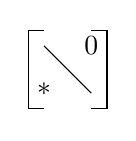
\begin{tikzpicture}
\node at (.2,.2) {*};
\node at (.8,.8) {0};
\draw[-] (.2,.8) to (.8,.2);
\draw[-] (0,0) to (0,1);
\draw[-] (0,0) to (.2,0);
\draw[-] (0,1) to (.2,1);
\draw[-] (1,0) to (1,1);
\draw[-] (.8,0) to (1,0);
\draw [-] (.8,1) to (1,1);
\end{tikzpicture}}} \pi 
\vcenter{\hbox{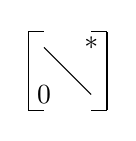
\begin{tikzpicture}
\node at (.2,.2) {0};
\node at (.8,.8) {*};
\draw[-] (.2,.8) to (.8,.2);
\draw[-] (0,0) to (0,1);
\draw[-] (0,0) to (.2,0);
\draw[-] (0,1) to (.2,1);
\draw[-] (1,0) to (1,1);
\draw[-] (.8,0) to (1,0);
\draw [-] (.8,1) to (1,1);
\end{tikzpicture}}}} = \overline{B_- \pi B_+} \subset \text{Mat}_n$$

For a linear representation $V$, the action $T \curvearrowright (V \supset X)$ gives us $[X \subset V] \in \text{Sym}T^{\ast} \simeq \Z[y_1, \dots, y_d]$.

Importantly, note that we can \textit{always} split $V$ as a direct sum of irreducible $T$-representations: \\
$$V \cong \bigoplus_{\text{weights }\lambda} \C_{\lambda}^{\oplus m_{\lambda}} \; \text{ for some multiplicities } m_{\lambda} \in \bN$$


Recall also our pipe dream formula, from yesterday's definition of the double Schubert polynomial $S_{\pi}$:
$$S_{\pi}(x_1, \dots, x_n, y_1, \dots, y_n) = [\overline{X_{\pi}} \subset \text{Mat}_n] = \sum_{\text{(pipe dreams for } \pi)} \prod_{\text{(crosses)}}x_{\text{row}} - y_{\text{col}}$$

\vspace{1em}

\begin{Definition}[Multigraded Hilbert series]
For a vector space $V$ of dimension $n$ (not necessarily equal to $\dim T)$, define $R \coloneqq \text{Fun}(V) \cong \C[z_1, \dots, z_n]$. Then the multigraded Hilbert series of $R$ is the formal sum
$$ h_R \coloneqq \sum_{\text{weights } \lambda \text{ of } T} \dim_{\C}(R_{\lambda})\, e^{\lambda}  \quad \in \mathbb{Z}[e^{\pm y_1}, \dots, e^{\pm y_d}]$$
where $R_{\lambda}$ is the $\lambda$-weight space of $R$.
\end{Definition}

Note that we have $h_{\oplus R_i} = \oplus h_{R_i}$.

To ensure the dimensions of the above weight spaces are finite, we impose the ``attractive condition" (we'll call it this, because we like it) that all $\lambda_i$ must lie in an open half-space.

\begin{Example}
We have the weight $\text{wt}(z_1^2 z_3) = -2 \lambda_1 - 1 \lambda_3$ (note that the coefficients are negative because we are acting on the dual space).
\end{Example}

\begin{Example}
For $n=1$, we have $\C[z_1] = \text{Fun}(V)$. So $h_R = \sum_{k=0}^{\infty} e^{-k \lambda_1} = \frac{1}{1-e^{-\lambda_1}}$.
\end{Example}

\begin{Example}
For general $n$, using the calculation directly above, we obtain $\C[z_1, \dots, z_n] \cong \C[z_1] \otimes \dots \otimes \C[z_n]$. So $h_R = \Pi_{i=1}^{n}  \frac{1}{1-e^{-\lambda_i}}$.
\end{Example}

\begin{Definition}[Multigraded / $T$-equivariant module]
If $R \curvearrowright M$, we say that $M$ is a multigraded (i.e. $T$-equivariant) module if:
\begin{itemize}
    \item $T \curvearrowright M$ (i.e. $M = \oplus_{\lambda \in T^{\ast}} M_{\lambda}$)
    \item $r \in R_{\lambda}, m \in M_{\mu} \implies rm \in M_{\lambda + \mu}$
\end{itemize} \end{Definition}

\begin{Definition}[Multigraded Hilbert series of an $R$-module $M$]
For $M$ a finitely generated $R$-module, we define 
$$ h_M \coloneqq \sum_{\text{weights } \lambda \text{ of } T} \dim(M_{\lambda}) \, e^{\lambda} $$
\end{Definition} 

Note from the definition above that the multigraded Hilbert series is so named because it is not graded by $\mathbb{Z}$ or $\mathbb{N}$, but by the weight lattice for $T$. Being multigraded is the same as having a torus action.

\begin{Example}
If $M = Rm$ (a free $R$-module with one generator), and $\text{wt}(m) = \lambda_m$, then $h_M = e^{\lambda_m} h_R$.
\end{Example}

A key example is the case $M = R/I$,  where $I$ is a $T$-invariant ideal, and $X = V(I)$. This motivates the next definition: notice that if $I=0$ (so $X$ is the entire space $V$), then we'd like $[V \subset V]$ to be 1. Directly above, though, we've already computed this to be a sum not equal to 1. The ``$K$-theoretical version" here will fix this issue.

\begin{Definition}
Letting $X = V(I)$, we have $[X \subset V]_K \coloneqq \frac{h_{R/I}}{h_R}$.
\end{Definition}

\begin{Theorem}
$[X \subset V]_K$ is a Laurent polynomial in $\{e^{\lambda}\}$.
\end{Theorem}
\begin{proof}
Sketch: If $R/I$ is a finitely generated module over a Noetherian ring $R$, and $I = (f_1, \dots, f_n)$, then there is a finite free resolution of $R/I$:
$$ 0 \to \dots \to \oplus_i R[\mu_i] \to R \to R/I \to 0 $$
So, this free resolution terminates, and the Hilbert series we want is an alternating sum of Hilbert series corresponding to the terms in the free resolution. Using that the series ``commutes with direct sum," and the fact that we've already computed series for single terms, we obtain a finite Laurent polynomial.
\end{proof}

\begin{Example}
If $X \subset V$ is a linear subspace, with $V = X \oplus X'$, then $[X \subset V]_K = \prod_{\mu \in X'}(1-e^{-\mu}) \in \Z[e^{\pm \mu}]$, whereas $[X \subset V] = \prod_{\mu \in X'} \mu \in \text{Sym}T^{\ast} = \Z[y_1, \dots, y_n]$.
\end{Example}

\noindent Next, let's check which axioms for $[X \subset V]$ are still satisfied by $[X \subset V]_K$:
\begin{enumerate}
    \item[\checkmark (0)] $[\{0\} \subset \{0\}]_K = 1$
    \item [\checkmark (2)] For a hyperplane $W = \{f=0\}$ with $X \subset W \subset V$, $[X \subset V]_K \coloneqq \frac{h_X}{h_V} = \frac{h_X}{h_W} \frac{h_W}{h_V} = [X \subset W]_K [W \subset V]_K$.
    \item[\checkmark (1)] With the setup above, and $X \subset V$, $X \not \subset W$, and $X$ reduced and irreducible, recall that $X = V(I)$ for $I$ a prime ideal $\iff$ $R/I$ is an integral domain.
    
    Letting $h_{X \cap W} \coloneqq h_{R/(I+(f))}$, we have exact sequence
    $$ 0 \to (R/I)f \hookrightarrow R/I \twoheadrightarrow R/(I + (f)) \to 0 $$
    This gives us an injection
    $$ 0 \to R/I \stackrel{\cdot f}{\to} (R/I)f \to 0 $$
    The second map $\cdot f$ above is an isomorphism of $R$-modules, but not in the multigraded sense. To fix this, we must introduce a shift by the weight $[e^{\wt(f)}]$, with $\wt(f) = -\wt(V(f)/W)$.
    Then, we indeed have $[X \subset V]_K = [X \cap W \subset W]_K$, and the axiom holds.
    
    \item[$\bigtimes$ \, (3)] This axiom no longer holds for $[X \subset V]_K$. For example, consider $R = \C[x,y]$, and $I = (x^2 - y^2)$. This is not a prime ideal; we can form quotients by $(x-y)$ or $(x+y)$, obtaining the following short exact sequence of    homogeneous graded $R$-modules:
    $$ 0 \to R/(x^2-y^2) \to R/(x-y) \oplus R/(x+y) \to R/(x,y) \to 0 $$
\centerline{\includegraphics[width=4in]{5.1.jpeg}}

\end{enumerate}
\vspace{1em}
\textbf{Question:} How do we relate $[X \subset V]$ and $[X \subset V]_K$?
\begin{Theorem}
Replace $\lambda$ by $\epsilon \lambda$, and take the leading term. That is:
$$ \lim_{\epsilon \to 0} \left( \frac{[X \subset V]_K}{\epsilon^{\text{codim}_v X}} \right) = [X \subset V] $$
\end{Theorem}

A last definition, which will soon be relevant:

\begin{Definition}[Subword complex]
If $Q$ is a word in the generators of a Coxeter group $W$, with $w \in W$, the subword complex $\Delta(Q,w)$ is a simplicial complex with vertices corresponding to the elements of $Q$.

A subword $F \subset Q$ is called a facet (i.e. a maximal face) precisely when $Q \setminus F$ is a reduced word for $w$.
\end{Definition}

\begin{Example}
Let $r_1$ be the transposition $(12) \in S_n$. Then $\Delta(121, r_1)$ (where $121$ is shorthand for $r_1 r_2 r_1$) is the simplicial complex pictured: \vspace{1em}

\centerline{\includegraphics[width=2in]{5.2.jpeg}}

Note that we index faces and vertices according to ``missing" letters in $Q$, and the complex above is homotopy equivalent to a point. Note also that the unpictured bottom edge, $-2-$ (i.e., $(23)$ in cycle notation), is \textit{not} a facet, because $r_2 = (23)$ is not a reduced word for $r_1$, whereas the other edges yield.
\end{Example}

\section{Lecture 6 (Allen Knutson)}

\section{Lecture 7 (Paul Zinn-Justin)}

\section{Lecture 8 (Paul Zinn-Justin)}

\section{Lecture 9 (Allen Knutson)}

\section{Lecture 10 (Allen Knutson)}

\section{Lecture 11 (Paul Zinn-Justin)}

\section{Lecture 12 (Paul Zinn-Justin)}

\section{Lecture 13 (Allen Knutson)}

\section{Lecture 14 (Paul Zinn-Justin)}

\section{Lecture 15 (Allen Knutson)}

\section{Lecture 16 (Allen Knutson)}

\section{Lecture 17 (Paul Zinn-Justin)}

\section{Lecture 18 (Paul Zinn-Justin)}

\end{document}
